\documentclass[11pt]{article}

\usepackage[paper=a4paper,margin=0.75in]{geometry}
\usepackage{setspace}
\usepackage{amsmath,amsfonts,amssymb,amsthm}
\usepackage{graphicx}
\usepackage{hyperref}
\usepackage{bbm}
{
	\newtheorem{assumption}{\textit{Assumption}}
	\newtheorem{definition}{\textit{Definition}}
	\newtheorem{theorem}{\textit{Theorem}}
}
\numberwithin{equation}{section}

\usepackage{fancyhdr}
\pagestyle{fancy}
\rhead{\today}
\lhead{Industrial Organisation Revision -- Lecture 3}

\newcommand\blfootnote[1]{%
	\begingroup
	\renewcommand\thefootnote{}\footnote{#1}%
	\addtocounter{footnote}{-1}%
	\endgroup
}

\begin{document}
\onehalfspacing

\section{Competition with Negotiated Prices}
\blfootnote{These notes are based on Howard Smith's lectures from the 2018-2019 academic year.\\
Of course, this is our interpretation of the material Howard presented. Good content is his; mistakes are ours.}

\vspace{-1cm}

\subsection{Introduction to NiN}

\textbf{Nash-in-Nash} (Horn Wolinsky 1988): the basic idea is one of a Nash equilibrium governing a number of Nash bargaining games. One way to think about NiN is buyers and sellers sending out uncoordinated representatives to a number of bilateral negotiations: each negotiation is cooperative, but the equilibrium is non-cooperative\footnote{The use of a cooperative bargaining solution does not sit well with some researchers, who prefer other models such as Rubinstein's alternating offers model. However, we know that the Rubinstein solution converges to the Nash bargaining solution as the length of periods shrinks to zero, and the result holds for NiN as well (see Collard-Wexler et al., 2018).}. The Nash bargaining games are played by buyers and suppliers, who are bilaterally connected and set prices to divide the surplus from the buyer-supplier exchange. The price externalities that multiple sellers connecting to the same buyer impose on each other will drive price towards an equilibrium. \\\\
Consider the following structure, where D is the buyer and U the seller:

\begin{center}
	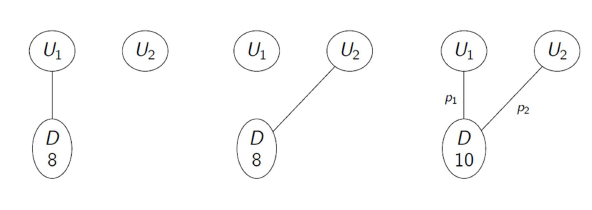
\includegraphics[width = 0.7\textwidth]{l2p1}
\end{center}

assume zero marginal cost and zero outside utility for the seller. It is evident that D will buy from both sellers iff their price is equal, and sellers have no reason not to sell at any strictly positive price. D has disagreement payoff 8 and agreement payoff 10 in both  Nash bargaining games. Her Nash bargaining solution is as follows:

\begin{equation*}
	p_1 = p_2 = p ~|~ \arg \max_p [(10-p) - 8][p] : 2 - 2p = 0 \rightarrow p = 1
\end{equation*}

Instead of assuming a disagreement payoff, one can endogenise it. Suppose for example D knows that she can buy at $p_e$ from $U_i$ if bargaining with $U_j$ fails ($i \neq j$), and has disagreement payoff $9 - p_e$. The Nash bargaining solution is

\begin{equation*}
	\underbrace{p_i = p_j = p}_{symmetry} ~|~ \arg \max_p [(10-p) - (9 - p_e)][p] : 1+p_e - 2p = 0
\end{equation*}
and note that in equilibrium $p_e = p$, so that $p_e = p = 1$ and $9 - p_e = 8$. A similar thought exercise can be conducted to estimate the impact of a \textbf{merger} between $U_1$ and $U_2$, which deprives D of a bargaining outside option, on price and, relatedly, on total welfare.

\subsection{Estimation of NiN }

Continue with the $\{U_i$, $U_j$, $D\}$ example. Set the beliefs as follows: if a bilateral exchange does not take place, agents expect the other trade to take place (\textit{passive beliefs}). Firms have marginal cost $mc_i$, D pays prices $p_i$.

D has payoff $\pi_{12}$ if she can agree with both sellers, $\pi_1$ if she can't agree with $U_2$, and $\pi_2$ if she can't agree with $U_1$. $\pi$ is a function of prices indicated by the subscript. Demands are denoted by $q_i(p_1,p_2)$.

The following payoff matrix applies for $i,j \in \{1,2\}, i \neq j $ given passive beliefs:

\begin{center}
	\begin{tabular}{ccc}
		&  $U_i$ & D \\
		$U_i$ and D agree & $q_i(p_1,p_2)(p_i - mc_i$) & $\pi_{12}$ \\
		$U_i$ and D disagree & 0 & $\pi_j$
	\end{tabular}
\end{center}

The Nash bargaining solution is
\begin{equation}
\label{nin}
p_i = \arg \max_{p_i} [\pi_{12} - \pi_j]^{b_D}[q_i(p_i - mc_i) - 0]^{b_{U_i}}
\end{equation}
Given $\ln(\cdot)$ is a strictly increasing function in the price domain, $p_i$ will also maximise
\begin{equation}
\label{lnnin}
p_i = \arg \max_{p_i} b_D \ln [\pi_{12} - \pi_j] + b_{U_i} \ln[q_i(p_i - mc_i) - 0]
\end{equation}
with first order condition
\begin{equation*}
	b_D \frac{\frac{\partial \pi_{12}}{\partial p_i} - \frac{\partial \pi_j}{\partial p_i}}{\pi_{12} - \pi_j} + b_{U_i}\frac{q_i + (p_i - mc_i) \frac{\partial q_i}{\partial p_i}}{q_i(p_i - mc_i)} = 0
\end{equation*}
which, by using $\frac{\partial \pi_{12}}{\partial p_i} = \frac{\partial \pi_i}{\partial p_i} = - q_i$ (proof in section on Grennan, 2013) and $\frac{\partial \pi_j}{\partial p_i} = 0$, yields
\begin{equation*}
	b_{U_i}\frac{q_i + (p_i - mc_i) \frac{\partial q_i}{\partial p_i}}{q_i(p_i - mc_i)} = b_D \frac{q_i }{\pi_{12} - \pi_j}
\end{equation*}
\begin{equation*}
	(p_i - mc_i) \frac{\partial q_i}{\partial p_i} = \frac{b_D}{b_{U_i}}\frac{q^2_i}{\pi_{12} - \pi_j}(p_i - mc_i) - q_i
\end{equation*}
\begin{equation}
\label{lnnineq}
	p_i = mc_i - q_i \underbrace{\bigg\{ \frac{\partial q_i}{\partial p_i} - \frac{b_D}{b_{U_i}}\frac{q^2_i}{\pi_{12} - \pi_j} \bigg\}^{-1}}_{\Omega(b)}
\end{equation}
where note that \eqref{lnnineq} reduces to Nash pricing if the buyer has no bargaining power ($b_D = 0$). \\

To make progress, we can:
\begin{enumerate}

\item Specify a functional form for $mc_i$:
\begin{equation}
\label{mc1}
	mc_i = w_i \gamma + \nu_i
\end{equation}
with, denoting by $z_i$ an instrument that allows identification of $b$ and assuming all elements of $\Omega$ except $b$ are known,
$ \mathbb{E}(\nu_i | w_i, z_i) \overset{\eqref{lnnineq}\eqref{mc1}}{=} \mathbb{E}(p_i + q_i \Omega(b) - w_i \gamma | w_i,z_i) = 0 $.

\item Assume a functional form depending on unobserved heterogeneity for the bargaining power ratio and let marginal costs be deterministic:
\begin{equation}
\label{mc2}
	\frac{b_D}{b_{U_i}} = \beta \nu_i \hspace{2cm} mc_i = w_i \gamma
\end{equation}
with $\mathbb{E}(\ln \nu_i | w_i, z_i) = 0$. Functional form \eqref{mc2} can in particular yield, with some rearranging, an isolated term for the bargaining power ratio\footnote{kids, if you assume everything is nicely multiplicative then you can take logs and isolate stuff!} (see below).
\end{enumerate}

\section{Application: Grennan (2013)}

An analysis of price discrimination, bargaining and the effect of merging purchasers in the market for coronary stents.
Two types of stent, one than can scar and one that does not.

\subsection{Setup}

Two-stage game: in the first stage, manufacturers and hospital $h$ negotiate stent prices for time $t$, $p_{ht}$; in the second stage, doctors decide which stent to assign to patients given prices and stent choice set. Backwards inducing,

\textbf{Stage 2}: Doctor chooses stent $j$ to maximise patient $i$'s utility with functional form
\begin{equation}
\label{u}
	u_{ijht} = \delta_{jht} + \epsilon_{ijht} \equiv \gamma_{jh} + \xi_{jht} - \alpha p_{jht} + \beta x_{jt} + \epsilon_{ijht} \hspace{2cm} \epsilon_{ijht} \sim \text{EVT-1}
\end{equation}
where $\gamma_{jh}$ is hospital-specific taste and $\xi_{jht}$ is a time-varying shock. \\
Non-stent treatment purchases are taken as excluded good. The market share and total demand of good $j$ are
\begin{equation}
\label{share}
	s_{jht} = \frac{e^{\delta_{jht}}}{\sum_{k \in J_{ht}} e^{\delta_{jht}}} \hspace{2cm} q_{jht} \equiv Q_{ht}s_{jht}
\end{equation}

\textbf{Stage 1}: The payoff to the hospital from choice set $J_{ht}$ is (using the standard EVT-1 result)
\begin{equation}
\label{payoffh}
	\pi (p_{ht}) = \frac{Q_{ht}}{\alpha} \mathbb{E}_\epsilon [\max_{j \in J_{ht}} (\delta_{jht} + \epsilon_{ijht})] = \frac{Q_{ht}}{\alpha} \ln [\sum_{j \in J_{ht}} e^{\delta_{jht}}]
\end{equation}
and, if choice $k$ is excluded, it is
\begin{equation}
	\pi_{-k} (p_{ht}) = \frac{Q_{ht}}{\alpha} \mathbb{E}_\epsilon [\max_{j \in J_{ht} \setminus k} (\delta_{jht} + \epsilon_{ijht})] = \frac{Q_{ht}}{\alpha} \ln [\sum_{j \in J_{ht} \setminus k} e^{\delta_{jht}}]
\end{equation}
$\pi_{-k} (p_{ht})$ is effectively the disagreement payoff each hospital gets if bargaining fails with producers of $k$: the added value of the additional stent type is $\pi(p_{ht}) - \pi_{-k} (p_{ht})$. Hospitals have passive beliefs. Stent sellers have 0 disagreement utility. Thus the Nash bargaining solution price is
\begin{equation}
  p_{jht} ~|~ \arg \max_{p_{jht}} ~ [\pi(p_{ht}) - \pi_{-j} (p_{ht})]^{b_{h}}[q_{jht}(p_{jht} - mc_{jht})]^{b_j}
\end{equation}
with first order condition
\begin{equation*}
	p_{jht} ~|~ \arg \max_{p_{jht}} ~b_h \ln [\pi(p_{ht}) - \pi_{-j} (p_{ht})] + b_j \ln [q_{jht}(p_{jht} - mc_{jht})]
\end{equation*}
\begin{equation*}
	b_j  \frac{\frac{\partial q_{jht}}{\partial p_{jht}}(p_{jht} - mc_{jht}) + q_{jht}}{q_{jht}(p_{jht} - mc_{jht})} = - 	b_h \frac{\frac{\partial \pi(p_{ht})}{\partial p_{jht}}}{\pi(p_{ht}) - \pi_{-j} (p_{ht})}
\end{equation*}
noting
\begin{equation*}
 \frac{\partial \pi_{ht}}{\partial p_{jht}} \overset{\eqref{payoffh}}{\equiv} \frac{Q_{ht}}{\alpha} \frac{\partial  \ln [\sum_{j \in J_{ht}} e^{\delta_{jht}}]}{\partial p_{jht}} \equiv \frac{Q_{ht}}{\alpha} \frac{\partial  \ln [\sum_{j \in J_{ht}} e^{\delta_{jht}}]}{\partial \sum_{j \in J_{ht}} e^{\delta_{jht}}} \frac{\partial \sum_{j \in J_{ht}} e^{\delta_{jht}}}{\partial p_{jht}} \equiv - Q_{ht} \frac{e^{\delta_{jht}}}{\sum_{j \in J_{ht}} e^{\delta_{jht}}} \overset{\eqref{share}}{=} - q_{jht}
\end{equation*}
one obtains
\begin{equation*}
b_j \bigg( 1 + \frac{\partial q_{jht}}{\partial p_{jht}} \frac{(p_{jht} - mc_{jht})}{q_{jht}} \bigg) = b_h \frac{q_{jht}(p_{jht} - mc_{jht})}{\pi(p_{ht}) - \pi_{-j} (p_{ht})}
\end{equation*}
\begin{equation*}
b_j \bigg( 1 + \frac{\partial q_{jht}}{\partial p_{jht}} \frac{(p_{jht} - mc_{jht})}{q_{jht}} \bigg) \frac{ \big(\pi(p_{ht}) - \pi_{-j} (p_{ht})\big)}{q_{jht}}= b_h (p_{jht} - mc_{jht})
\end{equation*}
finally add $b_j(p_{jht} - mc_{jht})$ to both sides and rearrange to obtain equation (8) in Grennan,
\begin{equation}
\label{grennan8}
	p_{jht} = mc_{jht} + \frac{b_j}{b_j + b_h} \bigg[\bigg( 1 + \frac{\partial q_{jht}}{\partial p_{jht}} \frac{(p_{jht} - mc_{jht})}{q_{jht}} \bigg) \frac{ \big(\pi(p_{ht}) - \pi_{-j} (p_{ht})\big)}{q_{jht}} + p_{jht} - mc_{jht} \bigg]
\end{equation}

Identification: bargaining generates two sources of demand identification: \textbf{(i)} negotiated prices depend on exogenous variation in bargaining abilities of players (see \eqref{grennan8}), i.e. bargaining ability is a supply shifter; \textbf{(ii)} if a contract fixes prices for a long period, price renegotiation will induce movement along the demand curve, thus allowing identification. Moreover, Grennan defines a functional form for unobserved time-changing hospital-level preferences $\xi_{jht}$, which is defined to be AR(1): $\xi_{jht} = \rho \xi_{jht-1} + \bar{\xi}_{jht}$.
As a result of the assumed exogeneity in bargaining ability variation and a timing assumption in the error term $\bar{\xi}_{jht}$, assumed to be realised after price setting, the author can then claim that prices in \eqref{u} are indeed exogenous.\footnote{``there is no simultaneity problem in using contemporaneous price as its own instrument'' (p. 158)} To avoid offending IV-heads, the author nonetheless instruments price with lagged price and within-hospital price average of other stents (a measure of hospital bargaining power).  \\

Given the simple logit formulation, \eqref{u} can then be estimated as
\begin{equation*}
	\ln s_{jht} - \ln s_{0ht} =  \gamma_{jh} + \xi_{jht} - \alpha p_{jht} + \beta x_{jt} + \epsilon_{ijht}
\end{equation*}

As for pricing equation estimation, note that the first order condition of the Nash bargaining problem would not allow to separately identify variation in marginal costs from variation in (the ratio of) bargaining powers. To circumvent the issue, the author assumes that
\begin{equation}
	mc_{jht} = mc_j = \mathbbm{1}_{\{j = scar\}}mc_{scar} + \mathbbm{1}_{\{j = noscar\}}mc_{noscar} \hspace{1cm} \text{and} \hspace{1cm} \frac{b_h}{b_j} = \beta_{jh}\nu_{jht}
\end{equation}
where $\nu$ is a random unobservable that drives the bargaining power disparity. These parametric assumptions can then be plugged into the \eqref{grennan8}, which one can then rearrange to obtain (cf. second-to-last step in deriving \eqref{grennan8})
\begin{equation}
	p_{jht} - mc_j = \beta_{jh}\nu_{jht} \underbrace{\bigg[\bigg( 1 + \frac{\partial q_{jht}}{\partial p_{jht}} \frac{(p_{jht} - mc_{j})}{q_{jht}} \bigg) \frac{ \big(\pi(p_{ht}) - \pi_{-j} (p_{ht})\big)}{q_{jht}}\bigg]}_{g(\cdot)}
\end{equation}
\begin{equation}
	\ln \frac{p_{jht} - mc_j}{g(\cdot)} = \ln \beta_{jh} + \ln \nu_{jht}
\end{equation}

Marginal costs and relative bargaining abilities are separately identified by the assumption of time-invariance of the former. Problem: changes in added value $g(\cdot)$ can be due to both to supply (marginal cost) and demand (eg. through $\pi_{-j}$) changes. If however demand does not change in response to anticipated changes in bargaining abilities, one can instrument added value with past values, resolving simultaneity. \\

Empirically, the author separately estimates the demand and supply parts of his model, using a GMM method \'{a} la Berry, Levinsohn and Pakes (1995).
For demand, one first matches predicted and realised market shares, inverts the equality to isolate doctor/patient heterogeneity estimates (Berry, 1994 shows there will be a unique solution), then estimates model parameters by GMM orthogonality conditions on $\xi_{jht}$; for supply, Grennan makes use of the parametric assumptions above and similarly estimates the supply unobservable $\nu$.

\subsection{Results}

Obtained own elasticities are $>-1$, consistent with buyers pushing prices in the inelastic part of demand:
\begin{center}
	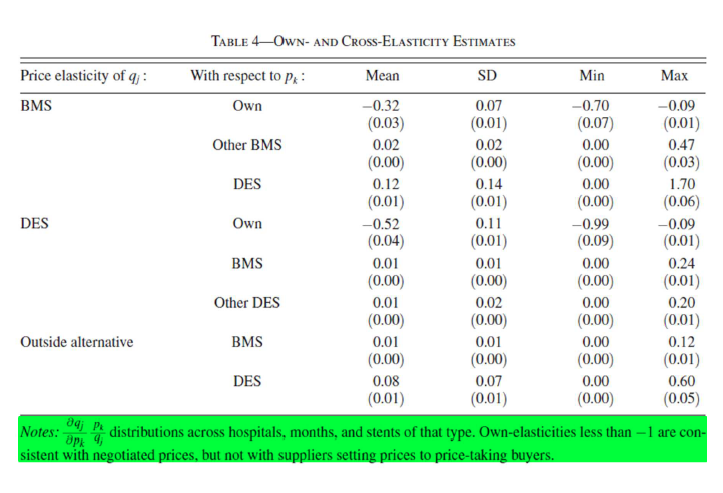
\includegraphics[width = 0.6\textwidth]{l3p2}
\end{center}
Moreover, cost estimates from the bargaining model seem to be reasonable (?), which cannot be said for Bertrand model estimates (\textit{negative} marginal costs):
\begin{center}
	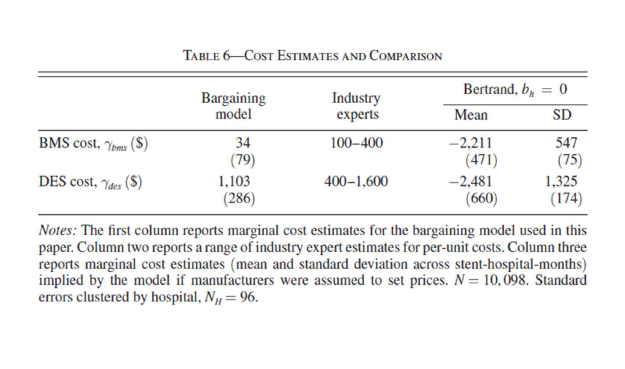
\includegraphics[width = 0.6\textwidth]{l3p3}
\end{center}
Lastly, the evidence from estimated changes in profits from switching to uniform pricing corroborates the evidence that allowing hospitals to team up in bargaining has positive effects on the public: forcing hospital bargaining power to zero would increase dramatically firm profits and shoot stent prices through the roof, reducing surplus for buyers.
\begin{center}
	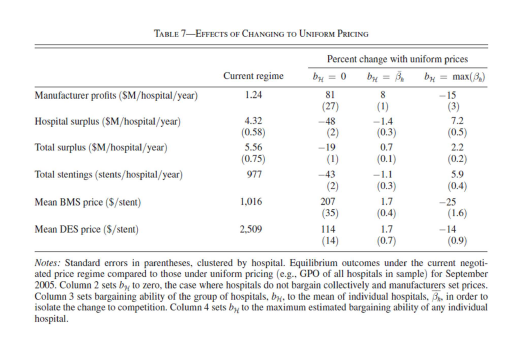
\includegraphics[width = 0.6\textwidth]{l3p4}
\end{center}


\end{document}
